\chapter{Discussion}

The $\alpha$ and $\beta$-phase of \ac{QA} on Ag(100) were investigated using \ac{XPS} for three different components: C1s, O1s and N1s. The ensuing discoure will meticulously examine the results obtained from \autoref{sec:results}, which will be methodically organized into discrete chapters to facilitate a comprehensive analysis of each phase.


\section{The 1D \texorpdfstring{$\alpha$}{alpha}-Phase}

The C1s \ac{XPS} spectra consist of four distinct components, corresponding to distinct carbon atoms in the \ac{QA} molecule, namely  $\mathrm{C_{arom}}$,  $\mathrm{C_{NH}}$,  $\mathrm{C_{CO}}$ and  $\mathrm{C_{O}}$.

The carbon atoms $\mathrm{C_{arom}}$ have the least influence from the functional groups. This leads to a \ac{BE} in the center of the spectrum. Due to the number of carbon atoms associated with this peak, the peak area is the most substantial, and the peak provides the primary contribution to the overall shape of the spectrum. The \ac{BE} of the peak appears to be realistic, as evidenced by its alignment with other molecular adsorbated on Ag(100), such as \ac{PTCDA}, which exhibit comparable values.\autocite{Bauer2014}

The peak corresponding to the carbon atoms adjacent to the amine, designated as $\mathrm{C_{NH}}$, is located at a slightly decreased \ac{BE} in comparison to the $\mathrm{C_{arom}}$ peak. This behavior of aromatic systems with amine functional groups inside, such as those found in pyridine, is typically observed.\autocite{Mendolicchio2019, Bagus2025}

The peak that arises due to beam damage ($\mathrm{N1_{damage}}$) has a shift in its \ac{BE} of around 2.20~\si{\eV}. This large difference indicates a drastic change in the chemical environment of the nitrogen atom. Compared to other shifts in the \ac{BE}, e.g. for the carbon atoms, the influence of other neighboring atoms are not enough to explain this change. For this reason, something different has to happen at the nitrogen atom due to beam damage.

A typical observed phenomena for the amine group is the deprotonation of the nitrogen atom. The deprotonation of amine groups in \ac{XPS} spectra was examined with a shift in the \ac{BE} of about 2-3~\si{\eV}.\autocite{Kang1990, Ruano2021}  This matches to the results found for the $\mathrm{N1_{damage}}$ peak, leading to the assumption that the x-ray beam deprotonates some of the nitrogen atom .

Last, the \ac{XPS} spectra for the O1s components are discussed. The \ac{BE} of the $\mathrm{O1}$ peak matches to similar systems, e.g. \ac{PTCDA} on Ag(100).\autocite{Bauer2014} The satellite peak, $\mathrm{O1_{sat}}$, observed for \ac{QA} was also measured for \ac{PTCDA}. The satellite peaks for the two adsorbates have similar shifts in their \acp{BE} and area ratios. This indicates that the results of the O1s \ac{XPS} spectra and the fit model is realistic.

In summary, the entirety of the peaks in the \ac{XPS} spectra adequately describe the molecular structure of \ac{QA} and are in accordance with the literature. In addition, the observed peaks in the \ac{XPS} spectra corroborate the structure model proposed by N. Humberg.\autocite{Humberg2024} The chemical environment of all nitrogen and oxygen atoms is identical within the structure model, because all oxygen atoms of one molecule form a hydrogen bond with the amine group of another molecule. This is evident from the \ac{XPS} spectra, which exhibit only a single peak for the corresponding atoms. Furthermore, the results indicates that all molecules in the structure have a similar chemical environment, which also matches to the structure model.

\section{Phase transition}

The examination of the phase transition was made with measuring a sequence of C1s \ac{XPS} spectra while increasing the sample temperature. This sequence shows in principle that the phase transition from the $\alpha$- to the $\beta$-phase occurs in a stepwise manner while heating the sample to 450~\si{K}. A close examination of the data reveals a transition in each peak from one spectrum to the next \ac{XPS} spectrum. This indicates that all molecules would undergo simultaneous and analogous changes.

While this assumption may be theoretically valid, it appears to be improbable. A more probable theory posits that the phase occurs for some molecules prior to others, resulting in a decreases of the $\alpha$-phase and an increase the $\beta$-phase. This observation aligns with the findings reported by N. Humberg.\autocite{Humberg2024} Nevertheless, the exact process of the phase transition can not be verified with the given data.

\section{The commensurate 2D \texorpdfstring{$\beta$}{beta}-Phase}

For the $\beta$-phase of \ac{QA} on Ag(100) one set of \ac{XPS} spectra for all photoemission lines were recorded. First, the C1s \ac{XPS} spectra are discussed.
The $\beta$-phase exhibits four distinct peaks, that correspond to the same carbon atoms as in the $\alpha$-phase. The relative position, with the $\mathrm{C_{arom}}$ in the center, the $\mathrm{C_{NH}}$ peak towards lower, the $\mathrm{C_{CO}}$- and the $\mathrm{C_{O}}$ peak towards higher \acp{BE}. The three peaks, $\mathrm{C_{arom}}$, $\mathrm{C_{CO}}$ and $\mathrm{C_{O}}$, have a similar shift in their \acp{BE}. This corresponds to similar changes in their chemical environment.

The lower \ac{BE} could be explained with stronger interactions between the Ag(100) surface and \ac{QA}. Thereby, the metal surface could donate electron density to the molecule, resulting in lower \acp{BE}. This process is also observed in literature and thus a valid explaination for the observed change in the \ac{BE}.\autocite{Moulder1993}

However, the change exhibited in the $\mathrm{C_{NH}}$ peak is distinct. The \ac{BE} remains constant during the phase transition; nevertheless, this phenomenon should not be interpreted in such a simplistic manner. Instead, it should be interpreted as a similar change in the \ac{BE} towards lower values due to a stronger interaction with the surface and then another effect that increases the \ac{BE} again. This process involves a change in the nitrogen atom bound to the $\mathrm{C_{NH}}$ atom. The bond between the carbon and nitrogen atoms has a significant impact on the electron density at the $\mathrm{C_{NH}}$ atom and could decrease the electron density. This decreased electron density results in an increase in the \ac{BE} of the carbon atom.

This leads to the subsequent discussion of the N1s \ac{XPS} spectra for the $\beta$-phase, where the one peak for both nitrogen atoms from the $\alpha$-phase divides into two different peaks. At the outset, the \ac{BE} of the $\mathrm{N1}$ peak undergoes a slight decrease in association with the phase transition. This decrease is less significant than that observed for the other atoms. This implies that the nitrogen atom, corresponding to the $\mathrm{N1}$ peak, exhibits a marginal increase in electron density, while the overall changes are analogous to those observed in the entire molecule. The observed increase in electron density may be attributed to enhanced interactions between the Ag(100) surface and \ac{QA}.

The second peak for the $\beta$-phase is precisely coincident with the position of the peak from the $\alpha$-phase, which corresponds to beam damage. It can be posited that the nitrogen atom corresponding to the $\mathrm{N2}$ peak has the equivalent chemical environment as the $\mathrm{N1_{damage}}$ peak. As previously stated, the $\mathrm{N1_{damage}}$ peak corresponds to a deprotonated nitrogen atom, a finding that aligns with the literature.\autocite{Kang1990, Ruano2021} This observation suggests the hypothesis that the observed $\mathrm{N2}$ peak corresponds to a deprotonated nitrogen atom as well.

This means that in each \ac{QA} molecule exactly one of the two amine groups is deprotonated due to the phase transition. The energy, needed for the deprotonation, has to be overcompensated by the different orientation and stronger interaction with the Ag(100) surface in the $\beta$-phase, because the $\beta$ is thermodynamically favored.\autocite{Humberg2024} It is conceivable that the deprotonated nitrogen bonds to the Ag(100) surface and donates electron density to the metal, which would lead to a stabilization of the phase. This process could then overcompensate the energy loss due to deprotonation.

The transition observed from a single peak in the $\alpha$-phase to two peaks in the $\beta$-phase was likewise detected in the O1s \ac{XPS} spectra. The \ac{BE} of the $\mathrm{O1}$ peak remains nearly constant. This phenomena is analogous to that observed for the nitrogen atoms. Consequently, it can be deduced that the nitrogen $\mathrm{N1}$ and the oxygen $\mathrm{O1}$ are the two atoms that interact with each other in the $\alpha$- and $\beta$-phase. These two atoms still have a hydrogen bond in the $\beta$-phase between the keto and the amine group, which leads to similar \acp{BE} for both phases.

The second peak in the O1s \ac{XPS} spectrum for the $\beta$-phase then corresponds to the other oxygen atom that interacts with the $\mathrm{N2}$ peak. This $\mathrm{O2}$ peak exhibits a lower \ac{BE} in comparison to the $\mathrm{O1}$ peak by 0.5~\si{\eV}. This corresponds to an increased electron density at the oxygen atom, which could be result of a missing hydrogen bond between the oxygen atom from one molecule and the hydrogen atom of an amine group from another molecule.

For the $\beta$-phase, both O1s peaks in the \ac{XPS} spectra have satellites. These are at 1~\si{\eV} higher \acp{BE} than the main peaks, which corresponds to a slight increase in the \ac{BE} difference between satellite and main peak compared to the $\alpha$-phase. This indicates that the shake-up process also changes between the two phases.

The experimental results from the \ac{XPS} spectra have to be compared to the structure model from N. Humberg.\autocite{Humberg2024} First, the structure of the $\beta$-phase is commensurate. This is also seen in the C1s \ac{XPS} spectra, because it shows precise positions for each of the carbon atoms. Altogether, the C1s \ac{XPS} spectra match to the structure model of the $\beta$-phase.

However, the O1s and N1s \ac{XPS} spectra contradict the structure model. The \ac{XPS} spectra show for both atom types two distinct peak with a  1~:~1 area ratio. This observation does not align with the structure model. According to N. Humberg\autocite{Humberg2024}, the structure of the $\beta$-phase has 1.5 hydrogen bonds per \ac{QA} molecule, which would correspond to two distinct peaks with an area ratio of 1.5~:~0.5 (3~:~1).

Apart from this, the change in \ac{BE} for the N1s \ac{XPS} spectra indicates that 1 of the two nitrogen atoms per molecule is deprotonated. This finding was also not taken into account for the structure model. Furthermore, the deprotonation of one of the two nitrogen atoms would lead to the fact, that 1.5 hydrogen bonds per molecule are not possible anymore.

The results of the experiments lead to a different structure model for the $\beta$-phase. Therefore, two theoretically possible structure models are depicted in \autoref{fig:models}, which match to the SPA-LEED image and STM results from N. Humberg.\autocite{Humberg2024} The structure models will be discussed in the following.

The first structure model is similar to the one of N. Humberg.\autocite{Humberg2024} The positions of the molecules are exactly the same and dimers are also formed. The most important change is the deprotonation of one of the nitrogen atoms per molecule. The most probable nitrogen atom for the deprotonation is the one that is not in between the molecules of the dimer, otherwise there would be no reason to form these dimers. In addition, high electron density at the deprotonated nitrogen atom and at the oxygen atom would repel each other. This results in two hydrogen bonds between the two molecules of the dimer, meaning one hydrogen bond per molecule. No further hydrogen bonds are formed in this structure.

The structure seems the prefered one but there are further aspects that need to be discussed. In model 1, the deprotonated nitrogen, which then has a high electron density, is opposite to the oxygen atom, which also has a high electron density. Usually, the negative charges should repel each other. Nevertheless, it is possible that the nitrogen and the oxygen atom change their height and approach the surface. This could increase the instance between the two atoms. Furthermore, both atoms could donate electron density to the Ag(100) surface, which should also decrease the repulsion.

\begin{figure}[htb]
	\centering
	\begin{subcaptionbox}{structure model 1}[0.49\linewidth]
		{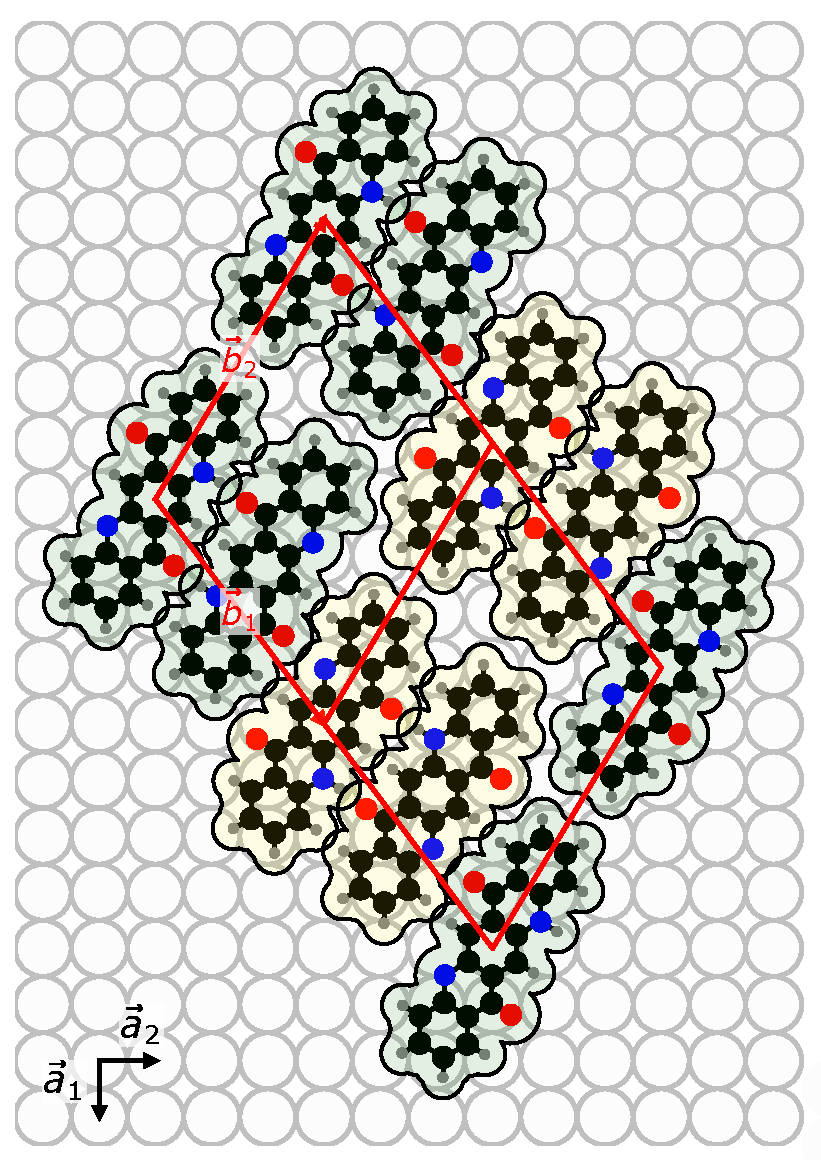
\includegraphics[width=\linewidth]{images/QA-beta-Ag(100)-Version1.pdf}}
	\end{subcaptionbox}
	\hfill
	\begin{subcaptionbox}{structure model 2}[0.49\linewidth]
		{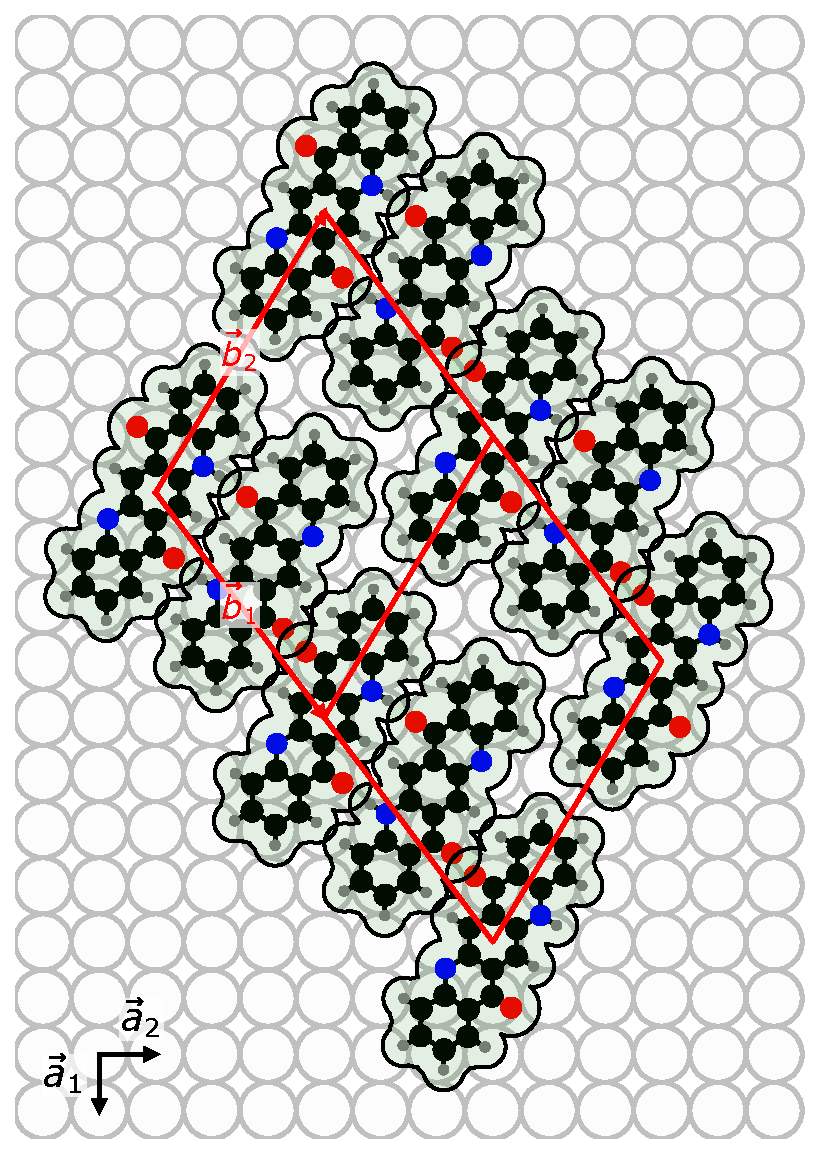
\includegraphics[width=\linewidth]{images/QA-beta-Ag(100)-Version2.pdf}}
	\end{subcaptionbox}
	\caption{Two different structure models for the $\beta$-phase of \ac{QA} on Ag(100).}
	\label{fig:models}
\end{figure}

The second structure model has more changes compared to the one of N. Humberg.\autocite{Humberg2024} Instead of the heterochiral dimers, the structure model is homochiral. This means that the molecules do not have to rotate on the surface for the phase transition from the $\alpha$- to the $\beta$-phase. The model also forms the same amount of hydrogen bridges as model 1.

However, a significant issue has been identified with model 2. As depicted in the structure model, the oxygen atom of one molecule is directly opposite to the oxygen atom of another molecule. The plausibility of this occurrence appears to be minimal, because they should also repel each other. It could also be possible that both oxygen atoms approach the surface and donate electron density to the surface. This could increase the distance between the atoms and decrease the repulsion. Nevertheless, model 2 appears to be less probable than model 1 for the reasons previously enumerated.

\cleardoublepage

